\chapter{Результаты работы}
\section{Архитектура системы}
Архитектура системы представляет собой модульную систему. Основными компонентами системы являются:
\begin{enumerate}
	\item TU webservice
	\item CoreService
	\item DataService
	\item Reasoner
	\item ClientAgent
	\item MessageBus
\end{enumerate}
Система может работать в 2-х режимах: режим обучения и режим запроса. Вариант использования для режима обучения представлен на Рисунке \ref{img:train}. Главными действующими лицами является специалист технической поддержки (TSS), в общем случае это базовый класс Пользователь (User). Данный вариант использования имеет несколько ветвей:
\begin{itemize}
	\item communication:Train - обучение посредством коммуникации с системой специалиста технической поддержки. 
	\item communication:ProvidesSolution - в случае коммуникации в режиме обучения специалист технической поддержки должен предоставить не только сам запрос, который будет формализован системой, но также решение данного запроса. Система формализует запрос, формализует решение и создаст между ними связи
	\item communication:ProvideRequest - специалист технической поддержки вводит в систему запрос
	\item communication:MonitorsSolution - специалист технической поддержки смотрит как применяется решение, если находится проблема, то решение корректируется в CorrectSystemSolutions
\end{itemize}
\begin{figure} [h] 
  \center
  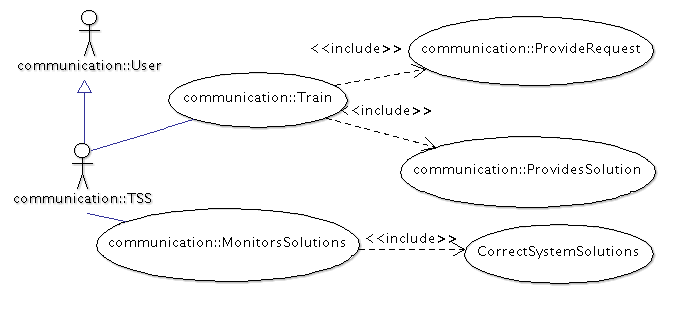
\includegraphics [scale=0.8, angle=90] {UseCaseTrain}
  \caption{Вариант использования. Обучение.} 
  \label{img:train}  
\end{figure}
Второй вариант использования это основной кейс. Главными действующими лицами системы является заказчик (Customer), в общем случае это базовый класс Пользователь (User). Он также имеет несколько ветвей:
\begin{itemize}
	\item ProvideRequest - заказчик вводит запрос в систему. Это может быть либо команда ProvideDirectInstruction, либо описание проблемы ProvideProblemDescription.
	\item communication:ProvideClarificationResponse - в случае, если система не может формализовать запрос, либо нашлось множество решений, то система запрашивает пользователя детали
	\item communication:ProvideConfirmationResponse - в случае, когда система нашла решение, она запрашивает пользователя подтверждение о том, что искомое решение решило его проблему
\end{itemize}
\subsection{Компоненты системы}
На Рисунке \ref{img:detailed_component_overview} представлена диаграмма компонентов системы. 
\begin{figure} [h] 
  \center
  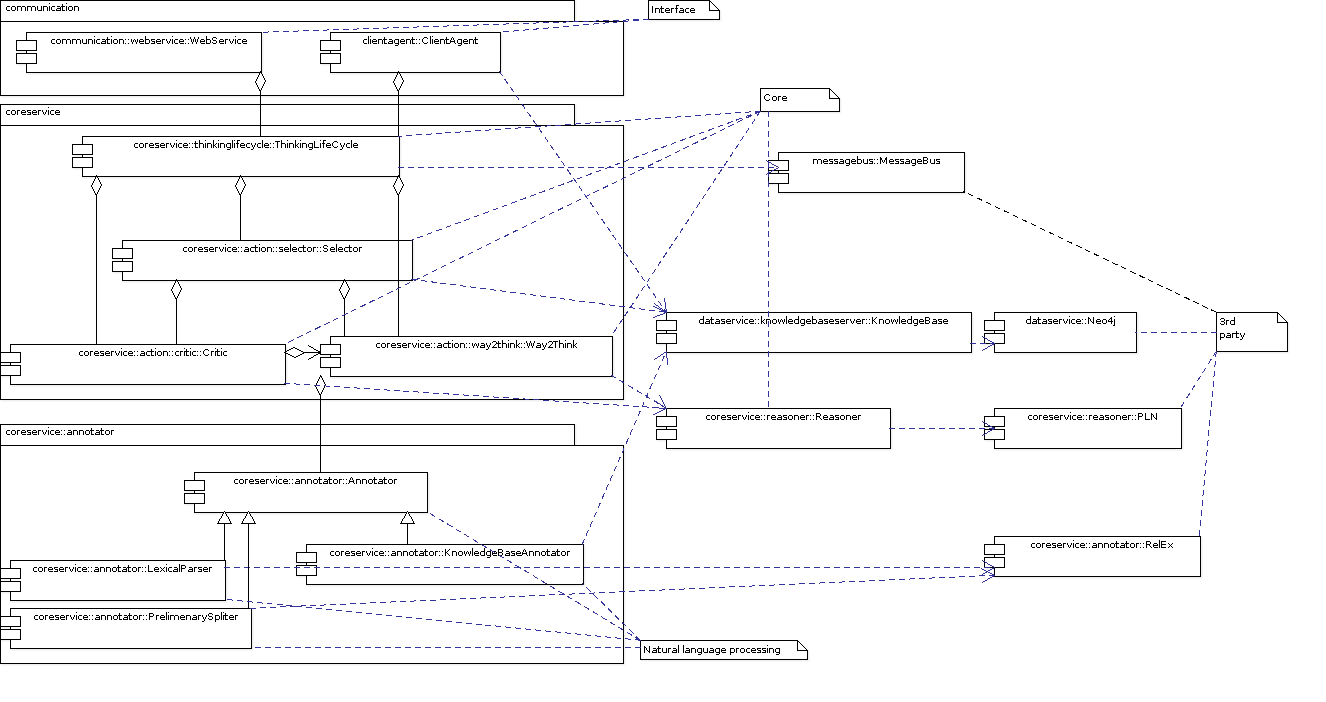
\includegraphics [scale=0.5, angle=90] {detailed_component_overview}
  \caption{Диграмма компонентов} 
  \label{img:detailed_component_overview}  
\end{figure}
Взаимодействие компонентов системы показано на рисунке \ref{img:main_components_collaboration}.
\begin{figure} [h] 
  \center
  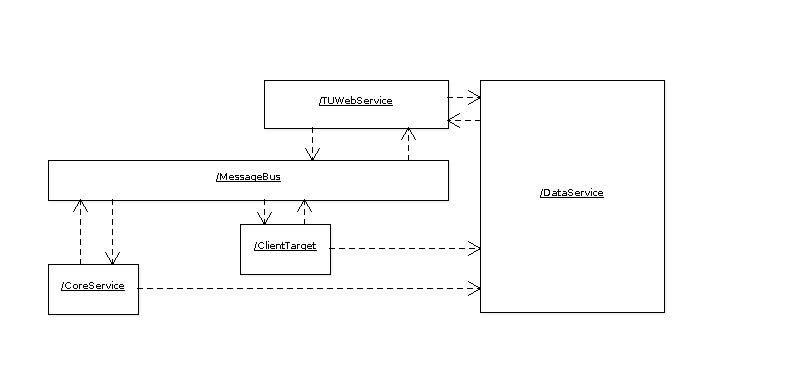
\includegraphics [scale=0.7] {main_components_collaboration}
  \caption{Диграмма взаимодействия компонентов} 
  \label{img:main_components_collaboration}  
\end{figure}
Пользователь взаимодействует с системой посредством компонента WebService \ref{WebService}. Взаимодействие происходит по следующем схеме:
\begin{enumerate}
	\item WebService получает запрос пользователя. Сохраняет запрос в Базу Знаний (Базу данных) \ref{Glossary}.
	\item WebService отправляет сообщение типа Request с информацией о запросе в компонент MessageBus (шина).
	\item Один из экземпляров CoreService компонента обрабатывает запрос.
	\item Компонент CoreService обрабатывает запрос и сохраняет результаты в Базу Знаний, затем он отправляет в MessageBus сообщение RequestCompleted и сообщение ActionsToExecute с действиями, которые необходимо исполнить
	\item WebService получает сообщение RequestCompleted c результатами выполнения запроса и уведомляет подписчиков (конечных пользователей)
	\item Компонент ClientAgent получает сообщение ActionsToExecute со списком действий, которые необходимо исполнить на целевых машинах
\end{enumerate}
\subsection{Компонент WebService} \label{WebService}
Данный компонент обрабатывает запросы пользователей. Запрос пользователя представляется объектом Request, который содержит информацию о пользователя, а также ссылку на метод, который будет вызван, когда запрос будет обработан. Вся работа происходит в компоненте CoreService.
На Рисунке \ref{img:web-service-interface} представлен интерфейс компонента.  
\begin{figure} [h] 
  \center
  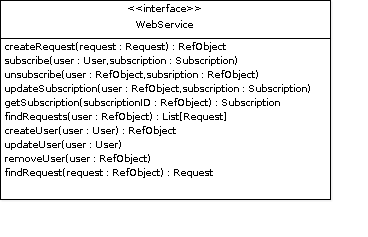
\includegraphics [scale=1.0] {web-service-interface}
  \caption{Интерфейс компонента WebService} 
  \label{img:web-service-interface}  
\end{figure}

\begin{table} [htbp]
   \centering
   \parbox{15cm}{\caption{Описание методов}\label{Methods Description}}
%  \begin{center}
  \begin{tabular}{| p{12cm} ||p{5cm} |}
  \hline
  \hline
Метод & Описание \\
  \hline
  createRequest(request:Request):[RefObject] & Создает запрос от пользователя. В качестве параметра в метод передается SubscriptionID, по которому идет проверка запроса. \\
  
  \hline
  subscribe(user:User,subscription:Subscription)  & Создает подписку для пользователя. \\
  \hline
  unsubscribe(user:RefObject,subscription:RefObject)   & Убирает подписку пользователя. \\
  \hline
  updateSubscription(user:RefObject,subscription:Subscription)   & Обновляет подписку пользователя. \\
  \hline
  getSubscription(subscriptionID:RefObject):List<Request>    & Возвращает подписку. \\
  \hline
  findRequests(user:RefObject)     & Возвращает запросы пользователя. \\
  \hline
  createUser(user:User):RefObject     & Создает пользователя. \\
  \hline
  updateUser(user:User)     & Обновляет информацию о пользователе. \\ 
  \hline
  removeUser(user:RefObject)     & Удаляет информацию о пользователе. \\ 
  \hline
  findRequest(request:RefObject):Request     & Возвращает запрос по ссылке. \\ 
  
  \hline
  \hline
\end{tabular}
%  \end{center}
\end{table}
Подробное описание классов представлено в \ref{AppendixA}. Основной алгоритм работы компонента:
\begin{enumerate}
	\item Пользователь создает запрос, используя метод WebService.createRequest
	\item Система сохраняет запрос в Базу Знаний и начинает его обработку
	\item Когда изменяется статус запрос request.state система оповещает подписчиков на этот запрос
\end{enumerate}
\subsection{Компонент CoreService.ThinkingLifeCycle}
Это основной компонент системы, ответственный непосредственно за выполнение запросов. Данный компонент управляет потоками, событиями приложения. Он запускает исполнение Критиков, Селекторов, Путей мышления, осуществляет обмен данных между компонентами. Компонент построен на фреймворке Akka Concurrency, который позволяет разрабатывать приложения, которые могут работать параллельно \cite{AkkaConcurrency}. \\
В данном компоненте реализовано шесть уровней мышления.
\begin{enumerate}
	\item Instinctive - Инстинктивный уровень
	\item Learned - Уровень обученных реакций
	\item Deliberative - Уровень рассуждений
	\item Reflective - Рефлексивный уровень
	\item Self-Reflective Thinking - Саморефлексивный уровень
	\item Self-Conscious Reflection - Самосознательный уровень
\end{enumerate}

На уровне Instinctive идет обработка сгенерированных по шаблону инцидентов.
Объект, который используется для обработки использует паттерн Akka \cite{AkkaConcurrency}. На рисунке \ref{img:thinking-life-cycle-cd} представлена диграмма классов компонента. 
\begin{figure} [h] 
  \center
  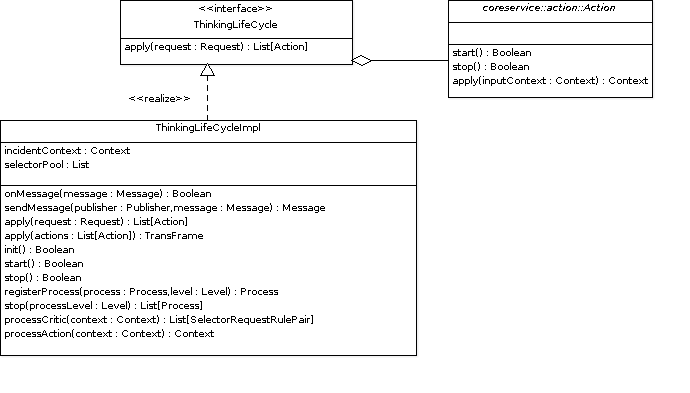
\includegraphics [scale=1.0,angle=90] {thinking-life-cycle-cd}
  \caption{Диаграмма классов ThinkingLifeCycle} 
  \label{img:thinking-life-cycle-cd}  
\end{figure}

\subsubsection{Описание методов класса}
\emph{onMessage(message : Message)} \\
Данный метод вызывается при получении сообщения от шины. После этого происходит обработка запроса, вычисляется список действий, которые нужно выполнить. После этого запускается исполнение этих действий. На рисунке \ref{img:thinking-life-cycle-on-message-ad} представлена диаграмма действий для этого метода.
\begin{figure} [h] 
  \center
  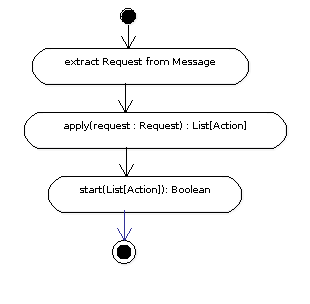
\includegraphics [scale=1.0] {thinking-life-cycle-on-message-ad}
  \caption{Диаграмма действий nnMessage} 
  \label{img:thinking-life-cycle-on-message-ad}  
\end{figure}

\emph{sendMessage(publisher: Publisher, message: Message): Boolean} \\
Данный метод используется для создания и отправки сообщения в шину. На рисунке \ref{img:thinking-life-cycle-send-message-publisher-publisher-ad} представлена диаграмма действий для этого метода.
\begin{figure} [h] 
  \center
  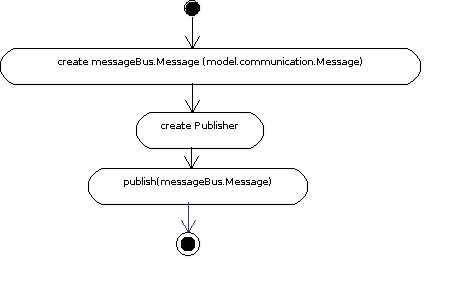
\includegraphics [scale=0.7] {thinking-life-cycle-send-message-publisher-publisher-ad}
  \caption{Диаграмма действий sendMessage} 
  \label{img:thinking-life-cycle-send-message-publisher-publisher-ad}  
\end{figure}

\emph{apply(request : Request) : List[Action]} \\
Данный метод используется для запуска обработки входящего запроса. Для запроса создается контекст, если такой уже не был создан. После этого вызывается следующий компонент системы Selector, который выбирает необходимые ресурсы из базы. На рисунке \ref{img:thinkinglifecycleapplyrequestRequestListAction} представлена диаграмма действий для этого метода.
\begin{figure} [h] 
  \center
  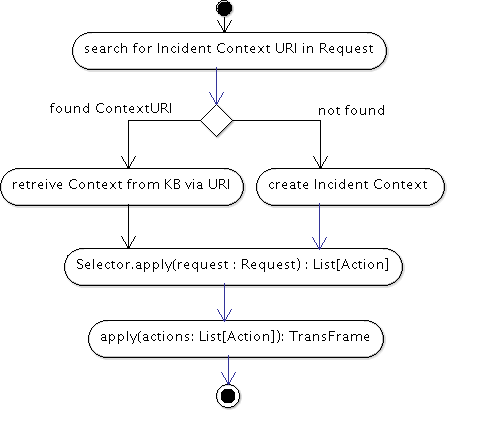
\includegraphics [scale=1.0] {thinkinglifecycleapplyrequestRequestListAction}
  \caption{Диаграмма действий apply} 
  \label{img:thinkinglifecycleapplyrequestRequestListAction}  
\end{figure}
Важно отметить, что метод apply является специальном методом в контексте функционального языка программирования Scala. По умолчанию при применение класса к параметрам исполняется функция apply \cite{ScalaProgrammingLanguage}.


\emph{apply(actions : List[Action]) : TransFrame} \\
Данный метод запускает обработку действий. Все действия разделяются на Critic (триггеры действий, которые в итоге должны перейти в WayToThink через Selector) и WayToThink (пути мышления, непосредственно обработчики данных, классы, которые производят изменения данных) На рисунке \ref{img:thinkinglifecycleapplyactionsListActionTransFrame} представлена диаграмма действий для этого метода.
\begin{figure} [h] 
  \center
  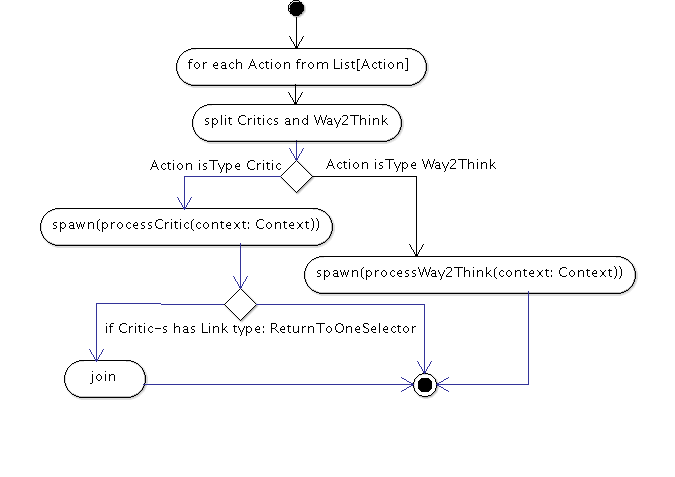
\includegraphics [scale=0.7] {thinkinglifecycleapplyactionsListActionTransFrame}
  \caption{Диаграмма действий apply} 
  \label{img:thinkinglifecycleapplyactionsListActionTransFrame}  
\end{figure}

\emph{processWay2Think(inputContext: Context, outputContext: Context): TransFrame} \\
Данный метод запускает обработку WayToThink \ref{Glossary}. Данный метод создает входной контекст (InputContext), заполняет его параметрами, создает выходной контекст OutputContext. Затем он запускает обработку данных во входном контексте. На рисунке \ref{img:thinkinglifecycleprocessWay2ThinkcontextContext} представлена диаграмма действий для этого метода.
\begin{figure} [h] 
  \center
  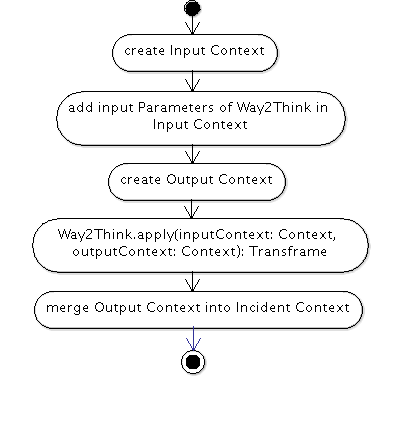
\includegraphics [scale=1.0] {thinkinglifecycleprocessWay2ThinkcontextContext}
  \caption{Диаграмма действий processWay2Think} 
  \label{img:thinkinglifecycleprocessWay2ThinkcontextContext}  
\end{figure}

\emph{processCritic(context: Context):List[SelectorRequestRulePair]} \\
Данный метод запускает обработку Critic \ref{Glossary}. На рисунке \ref{img:thinkinglifecycleactivityprocessCriticcontextContext} представлена диаграмма действий для этого метода.
\begin{figure} [h] 
  \center
  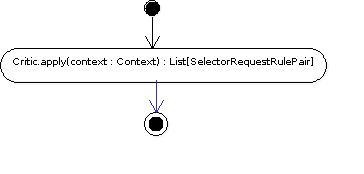
\includegraphics [scale=1.0] {thinkinglifecycleactivityprocessCriticcontextContext}
  \caption{Диаграмма действий processCritic} 
  \label{img:thinkinglifecycleactivityprocessCriticcontextContext}  
\end{figure}

\emph{init(): Boolean} \\
Данный метод инициализирует экземпляр класса ThinkingLifeCycle. Во время инициализации происходит Базы Знаний \ref{Glossary}, подключения к Шине данных. На рисунке \ref{img:thinkinglifecycleinitBoolean} представлена диаграмма действий для этого метода.
\begin{figure} [h] 
  \center
  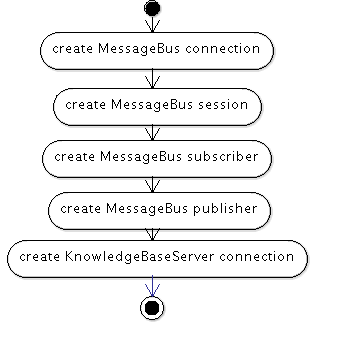
\includegraphics [scale=1.0] {thinkinglifecycleinitBoolean}
  \caption{Диаграмма действий init} 
  \label{img:thinkinglifecycleinitBoolean}  
\end{figure}

\emph{start(): Boolean} \\
Данный метод является оберткой для поддержки Akka Concurrency. Он вызывает метод init. 

\emph{stop(): Boolean} \\
Данный метод является оберткой для поддержки Akka Concurrency. Он останавливает работу экземпляра класса: останавливается сессия к шине данных, останавливается подключение к Базе Знаний. 

\emph{registerProcess(process : Process,level : Level) : Process} \\
Данный метод регистрирует процесс в пуле. В качестве параметра принимается Level (уровень приоритета процесса). 

\emph{stop(processLevel : Level) : List[Process]} \\
Данный метод регистрирует останавливает процесс. В качестве параметра принимается ссылка на процесс. На рисунке \ref{img:thinkinglifecyclestopprocessLevelLevelListProcess} представлена диаграмма действий для этого метода.
\begin{figure} [h] 
  \center
  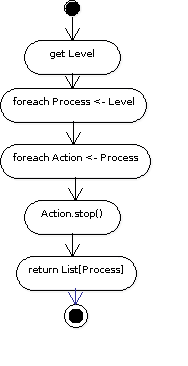
\includegraphics [scale=1.0] {thinkinglifecyclestopprocessLevelLevelListProcess}
  \caption{Диаграмма действий stop} 
  \label{img:thinkinglifecyclestopprocessLevelLevelListProcess}  
\end{figure}

\subsubsection{Описание работы компонента}
\emph{Запуск и остановка} \\
\begin{enumerate}
	\item Когда приложение стартует оно инициализирует ThinkingLifeCycle, который активирует набор критиков, базируясь на текущей цели системы. Например, цель-классифицировать инцидент, активируется набор критиков: разобрать, проверить, найти категорию.
	\item Когда приложение останавливается - оно останавливает все объекты класса и подклассов Actions (Critics, WayToThink), Selectors и ThinkingLifeCycle.
\end{enumerate}
Коммуникация происходит посредством сообщений, отправленных через MessageBus (Шину Данных) \ref{Glossary} JMS \cite{JMS}.
\emph{Взаимодействие компонента с другими компонентами} \\
\begin{enumerate}
	\item Критик возвращает список Селекторов (SelectorRequestRule)
	\begin{enumerate}
	\item ThinkingLifeCycle запускает обработку компонента Selector
	\item Selector возвращает список Action \ref{AppendixB} из базы знаний
	\item ThinkingLifecycle параллельно запускает возвращенные Action
	\begin{enumerate}
	\item Если Action это Critic
	\item ThinkingLifeCycle создает InputContext (входной контекст приложения) и копирует туда все данные из Context (контекста) инцидента
	\item Если Action это Critic с ссылками ReturnToSameSelector ThinkingLifeCycle ждет результаты и отправляет список SelectorRequestRule, возвращенные Critic новому Selector. Иными словами Critic может вернуть новый Selector. В данном случае нам нужно провести операцию Join для всех потоков \cite{JavaConcurrency}. В иных же случаях все Action запускаются в параллельных потоках.
	\end{enumerate} 
	\begin{enumerate}
	\item Если Action это WayToThink
	\item ThinkingLifeCycle создает InputContext (входной контекст приложения) и копирует туда все данные из Context (контекста) возвращенный Selector
	\item TLC \ref{Glossary} запускает WayToThink
	\item TLC сохраняет параметры в OutputContext
	\item TLC сохраняет итоговый результат работы и возвращает его 
	\end{enumerate} 
	\end{enumerate}
\end{enumerate}
\subsection{Компонент CoreService.Selector}
Selector это компонент, который ответственен за получение списка действий из Базы знаний, согласно входным параметрам.
\bold{Входной критерий}. TLC запускает Selector c параметрами. \\
\bold{Выходной критерий}. Selector получает список Action: WayToThink или Critic. \\
 
\subsection{Компонент CoreService.Critics}
\subsection{Компонент CoreService.Way2Think}
\subsection{Компонент CoreService.PreliminaryAnnotator}
\subsection{Компонент CoreService.KnowledgeBaseAnnotator}
\subsection{Компонент CoreService.Link parser}
\section{Прототип}
\section{Испытание прототипа}
\section{Выводы по главе}
%\newpage
%============================================================================================================================


\clearpage